\documentclass[12pt]{elsart}
\usepackage{amsmath}
\usepackage{amssymb}
\usepackage{program}
\usepackage{graphicx}
\usepackage{cancel}
\newcommand{\field}[1]{\mathbb{#1}}
\usepackage[letterpaper,top=0.75in, bottom=0.75in, left=1in, right=1in]{geometry}


\usepackage{algorithm}
\usepackage{algpseudocode}

%%%%%%%%%%%%%%%%%%%%%%%%%%%%%%%%%%%%%%%%%Space to make more readable!
%\vspace{10 mm}
%%%%%%%%%%%%%%%%%%%%%%%%%%%%%%%%%%%%%%%%%Take out later!

\begin{document}
Bryan Burkhardt - XMV643\\
CS3343 Section 01\\
04 Nov 2017\\

\pagestyle{empty}

\begin{center}
\Large  CS3343 Analysis of Algorithms Fall 2017 \\
\large {\bf Homework 6}\\
\normalsize Due 11/3/17 before 11:59pm (Central Time)
\end{center}

{\bf 1.  Franchise Restaurants (5 points)}

A fast food company is considering a bunch of bids to open franchises on a road and they want to develop an algorithm to decide which to accept.

For each of the $n$ miles along the road, the bid for that location is recorded (if there is no bid it is recorded as $0$).  The company wants to accept the bids which maximizes their total earnings.  One extra caveat is that two franchises must be at least $3$ miles apart (for example if you accept the bid at mile $5$ then you can't accept the bids at miles $3,4,6,7$).

\hspace*{0.5cm}  \begin{tabular}{ |l|l|l|l|l|l|l|l|l|l| }
  \hline
   Mile: & 1 & 2 & 3 & 4 & 5 & 6 & 7 & 8 & 9 \\
  \hline
  Bid: &   50,000 & 60,000 & 30,000 & 45,000 & 40,000 & 10,000 & 40,000 & 0 & 45,000 \\
  \hline
$E(i)$ & 50,000 & 60,000 & 60,000 & 95,000 & 100,000 & 100,000 & 135,000 & 135,000 & 145,000 \\
  \hline
\end{tabular}

   \begin{enumerate}
      \item (1 point) Example:  For the bids given above, which would you accept to maximize the earnings? (in this case, $n=9$)\\\\
	{\bf Answer:}\\
	After calculating $E(i)$, I would choose mile 2, 5, and 9 for a max profit of 145,000\\
      \item (2 points) Let $E(n)$ denote your maximum earnings for the bids in the first $n$ miles.  Give a recursive definition of $E$:
   \begin{enumerate}
      \item Base case \\(Hint: this will occur when $n=0$ since there are no bids to consider).\\\\
	\boxed{$if $ n==0 $ then $ E(n)=0}\\
      \item Recursive case \\(Hint: compare the total value obtained from accepting the $n\textsuperscript{th}$ bid to the total value obtained from not accepting the $n\textsuperscript{th}$ bid).\\\\
	$E(n) = max(b(n)+E(n-3), E(n-1))$\\
	return $max(E(n), E(n-1))$\\
   \end{enumerate}
\newpage
      \item (2 points) Give pseudo-code for an algorithm which uses memoization to compute $E(n)$ based on the above recurrence (assume you are passed an array $b$ of the bids).\\\\
	\begin{algorithm}
	\caption{int memoization(int n, int[] b)}
	\begin{algorithmic}
	\State Create new array E of size n, initialize each index to null
	\State memoization(n, b, E);
	\end{algorithmic}
	\end{algorithm}
	\begin{algorithm}
	\caption{int memoization(int n, int[] b, int[] E)}
	\begin{algorithmic}
	\If {E[n]==null}
		\If {n==0}
		\State E[n]=0;
		\Else
		\State E[n]=max(b[n]+memoization(n-3,b,E), memoization(n-1,b,E));
		\EndIf
	\EndIf
	\State return E[n];
	\end{algorithmic}
	\end{algorithm}
	
   \end{enumerate}

{\bf 2.  Inventory Management (7 points)}

Suppose you are playing a video game.  In this game you can only carry a limited amount of items.  Every item has a value and your goal is to maximize the total value of items you are carrying.  

Specifically, you are choosing which of $m$ items to carry where item number $i$ has value $v[i]$ (for your recurrence/pseudo-code you can assume you are passed the item values  in an array, $v$, of size $m$).  

\begin{enumerate}
   \item Suppose you can only carry $n$ items of the $m$ available.
   \begin{enumerate}
      \item (1 point) Example: Let $n=3$, $m=5$.  If the item values are $v=\{5,30,17,32,40\}$ which $3$ should you choose to carry?\\\\
	{\bf Answer:}\\
	Item 2, 4, and 5 for a combined value of 102\\
      \item (1 point) Give a short description of a greedy algorithm which maximizes your total value for any given $n$,$m$, and $v$.\\\\
	{\bf Answer:}\\
	Grab the first $n$ values from $v$ then compare each following value and replace the smallest grabbed value if the current $n$ is bigger.\\\\
   \end{enumerate}
\newpage
   \item Suppose, the game is updated so that every item, $i$, now has weight, $w[i]$, in kilograms (you can assume you are passed the item weights in an array, $w$, of size $m$).  You can only carry $n$ kilograms of weight.
   \begin{enumerate}
      \item (1 point) Example: Let $n=15$, $m=5$.  If the item values are $v=\{5,30,17,32,40\}$ and the item weights are $w=\{2,4,3,6,15\}$ which should you choose to carry?  Which would your greedy algorithm choose to carry?  \\\\
	{\bf Answer:}\\
	I would choose item 1, 2, 3, and 4 for a combined value of 84 and weight of 15. My greedy algorithm would end up grabbing item 5 for a value of 40 and weight of 15.\\\\
      \item (2 points) Let $V(n,m)$ denote your maximum total value for any given $n$, $m$, $v$, and $w$.  Give a recursive definition of $V$:
   \begin{enumerate}
      \item Base case \\(Hint: your base case will occur when $m=0$ since you have no items left to consider).\\\\
		\boxed{$if $m==0 $ then $ v[0] = 0}\\
      \item Recursive case \\(Hint: compare the total value obtained from taking the $m\textsuperscript{th}$ item to the total value obtained from not taking the $m\textsuperscript{th}$ item).\\\\
	$\boxed{$V[n,m]==max(V[n, m-1], V[n-w[m], m-1]+v[m])$}$\\
   \end{enumerate}
      \item (2 points) Based on your recurrence, write the pseudo-code for a dynamic programming algorithm to compute the maximum total value (you can use bottom up dynamic programming or memoization).
   \end{enumerate}
\end{enumerate}

{\bf 3.  DFS and BFS (6 points)}

For the following problems, assume that vertices are ordered alphabetically in the adjacency lists (thus you will visit adjacent vertices in alphabetical order).

   \begin{enumerate}
      \item (2 points) Execute a Breadth-First Search on the graph $G_1$, starting on vertex $a$. Specifiy the visit times for each node of the graph.\\\\
\hspace*{0.5cm}  \begin{tabular}{ |l|l|l|l|l|l|l| }
  \hline
   Visit Time: & 0 & 1 & 2 & 3 & 4 & 5 \\
  \hline
  Node: & a & c & f & e & b & d \\
  \hline 
\end{tabular}\\
      \item (2 points) Execute a Depth-First Search on the graph $G_1$, starting on vertex $a$. Specifiy the visit and finish times for each node of the graph\\\\
\hspace*{0.5cm}  \begin{tabular}{ |l|l|l|l|l|l|l| }
  \hline
   Node: & a & b & c & d & e & f \\
  \hline
   Visit Time: & 0, 11 & 4, 5 & 1, 10 & 3, 6 & 2, 9 & 7, 8 \\
  \hline 
\end{tabular}\\
   \begin{enumerate}
      \item (1 point) For each edge in your graph identify whether it is a tree edge, back edge, forward edge, or a cross edge.\\\\
  \hspace*{0.5cm}  \begin{tabular}{ |l|l|}
  \hline
   {\bf Edge} & {\bf Type:}  \\
  \hline
   a $\rightarrow$ c & tree, forward \\
  \hline 
   a $\rightarrow$ f & forward \\
\hline
c $\rightarrow$ e & tree, forward \\
\hline
e $\rightarrow$ d & tree, forward \\
\hline
e $\rightarrow$ f & forward \\
\hline
d $\rightarrow$ b & tree, forward \\
\hline
f $\rightarrow$ b & cross \\
\hline
b $\rightarrow$ a & back \\
\hline
\end{tabular}\\
      \item (1 point) Which edges would you remove to make your graph into a DAG?  (hint: use your edge classification to justify your choice)\\\\
{\bf Answer:}\\
I would remove the edge b $\rightarrow$ a because it's a back edge. According to the theorem in class, it states a directed graph G is acyclic $\Leftrightarrow$ a DFS yeilds no back edges.\\
   \end{enumerate}

   \end{enumerate}


{\bf 4.  Prim's Algorithm (4 points)}

(4 points) Run Prim’s algorithm on the graph $G_2$, with start vertex $a$. Assume that vertices are ordered alphabetically. 

For each step of the algorithm specify the current vertex weights (you can use a table to represent this data).  Draw the minimum spanning tree the algorithm finds. 

\hspace*{0.5cm}  \begin{tabular}{ |l|l|l|l|l|l|l| }
\hline
{\bf a} & {\bf b} & {\bf c} & {\bf d} & {\bf e} & {\bf f} & {\bf g} \\ 
  \hline
 0 & $\infty$ & $\infty$ & $\infty$ & $\infty$ & $\infty$ & $\infty$ \\
  \hline 
& 2 & $\infty$ & $\infty$ & $\infty$ & 11 & 5 \\
\hline
& & 8 & $\infty$ & $\infty$ & 11 & 4 \\
\hline
 &  & 7 & 15 & 6 & 11 &  \\
\hline
 &  & 7 & 1 &  & 3 &  \\
\hline
 &  & 7 & &  & 3 &  \\
\hline
 &  & 7 & &  &  &  \\
\hline
 &  & & &  &  &  \\
\hline
\end{tabular}\\
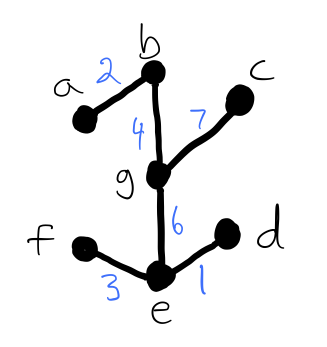
\includegraphics[scale=1]{prim.png}\\
\begin{figure}[h]
	\centering \includegraphics[width=.45\textwidth]{Graph-01}
\end{figure}


\end{document}